\chapter{Complete search}

\key{Compelete search}
is a general method that can be used
for solving almost any algorithm problem.
The idea is to generate all possible
solutions for the problem using brute force,
and select the best solution or count the
number of solutions, depending on the problem.

Complete search is a good technique
if it is feasible to go through all the solutions,
because the search is usually easy to implement
and it always gives the correct answer.
If complete search is too slow,
greedy algorithms or dynamic programming,
presented in the next chapters,
may be used.

\section{Generating subsets}

\index{subset}

We first consider the case where
the possible solutions for the problem
are the subsets of a set of $n$ elements.
In this case, a complete search algorithm
has to generate
all $2^n$ subsets of the set.

\subsubsection{Method 1}

An elegant way to go through all subsets
of a set is to use recursion.
The following function \texttt{gen}
generates the subsets of the set
$\{1,2,\ldots,n\}$.
The function maintains a vector \texttt{v}
that will contain the elements in the subset.
The generation of the subsets
begins when the function
is called with parameter $1$.

\begin{lstlisting}
void gen(int k) {
    if (k == n+1) {
        // process subset v
    } else {
        gen(k+1);
        v.push_back(k);
        gen(k+1);
        v.pop_back();
    }
}
\end{lstlisting}

The parameter $k$ is the number that is the next
candidate to be included in the subset.
The function branches to two cases:
either $k$ is included or it is not included in the subset.
Finally, when $k=n+1$, a decision has been made for
all the numbers and one subset has been generated.

For example, when $n=3$, the function calls
create a tree illustrated below.
At each call, the left branch doesn't include
the number and the right branch includes the number
in the subset.

\begin{center}
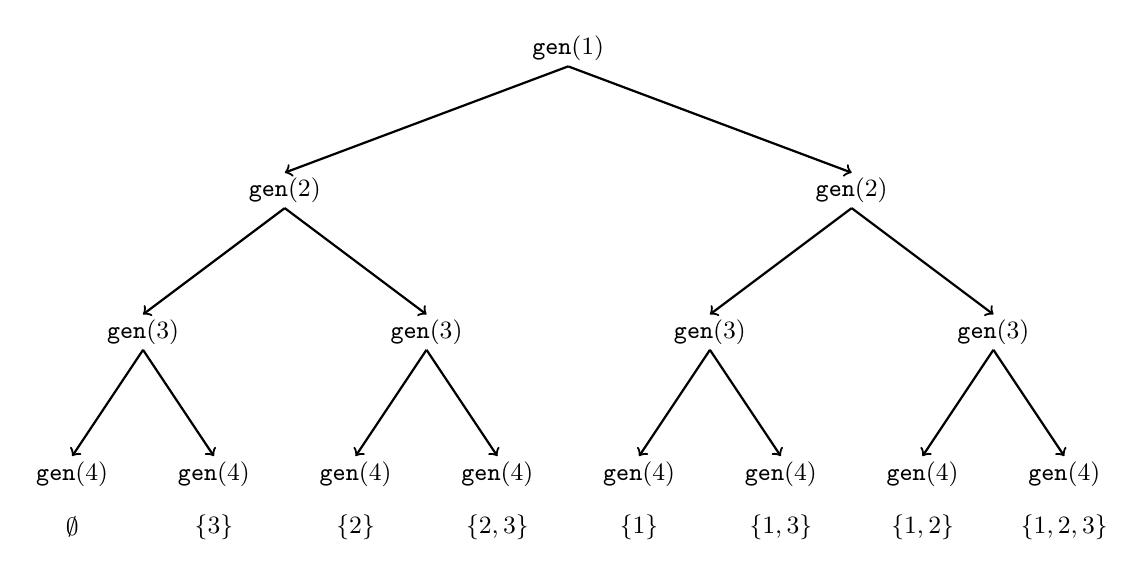
\begin{tikzpicture}[scale=.45]
  \begin{scope}
    \small
    \node at (0,0) {$\texttt{gen}(1)$};

    \node at (-8,-4) {$\texttt{gen}(2)$};
    \node at (8,-4) {$\texttt{gen}(2)$};

    \path[draw,thick,->] (0,0-0.5) -- (-8,-4+0.5);
    \path[draw,thick,->] (0,0-0.5) -- (8,-4+0.5);

    \node at (-12,-8) {$\texttt{gen}(3)$};
    \node at (-4,-8) {$\texttt{gen}(3)$};
    \node at (4,-8) {$\texttt{gen}(3)$};
    \node at (12,-8) {$\texttt{gen}(3)$};

    \path[draw,thick,->] (-8,-4-0.5) -- (-12,-8+0.5);
    \path[draw,thick,->] (-8,-4-0.5) -- (-4,-8+0.5);
    \path[draw,thick,->] (8,-4-0.5) -- (4,-8+0.5);
    \path[draw,thick,->] (8,-4-0.5) -- (12,-8+0.5);

    \node at (-14,-12) {$\texttt{gen}(4)$};
    \node at (-10,-12) {$\texttt{gen}(4)$};
    \node at (-6,-12) {$\texttt{gen}(4)$};
    \node at (-2,-12) {$\texttt{gen}(4)$};
    \node at (2,-12) {$\texttt{gen}(4)$};
    \node at (6,-12) {$\texttt{gen}(4)$};
    \node at (10,-12) {$\texttt{gen}(4)$};
    \node at (14,-12) {$\texttt{gen}(4)$};

    \node at (-14,-13.5) {$\emptyset$};
    \node at (-10,-13.5) {$\{3\}$};
    \node at (-6,-13.5) {$\{2\}$};
    \node at (-2,-13.5) {$\{2,3\}$};
    \node at (2,-13.5) {$\{1\}$};
    \node at (6,-13.5) {$\{1,3\}$};
    \node at (10,-13.5) {$\{1,2\}$};
    \node at (14,-13.5) {$\{1,2,3\}$};


    \path[draw,thick,->] (-12,-8-0.5) -- (-14,-12+0.5);
    \path[draw,thick,->] (-12,-8-0.5) -- (-10,-12+0.5);
    \path[draw,thick,->] (-4,-8-0.5) -- (-6,-12+0.5);
    \path[draw,thick,->] (-4,-8-0.5) -- (-2,-12+0.5);
    \path[draw,thick,->] (4,-8-0.5) -- (2,-12+0.5);
    \path[draw,thick,->] (4,-8-0.5) -- (6,-12+0.5);
    \path[draw,thick,->] (12,-8-0.5) -- (10,-12+0.5);
    \path[draw,thick,->] (12,-8-0.5) -- (14,-12+0.5);
\end{scope}
\end{tikzpicture}
\end{center}

\subsubsection{Method 2}

Another way to generate the subsets is to exploit
the bit representation of integers.
Each subset of a set of $n$ elements
can be represented as a sequence of $n$ bits,
which corresponds to an integer between $0 \ldots 2^n-1$.
The ones in the bit representation indicate
which elements of the set are included in the subset.

The usual interpretation is that element $k$
is included in the subset if $k$th bit from the
end of the bit sequence is one.
For example, the bit representation of 25
is 11001 that corresponds to the subset $\{1,4,5\}$.

The following iterates through all subsets
of a set of $n$ elements

\begin{lstlisting}
for (int b = 0; b < (1<<n); b++) {
    // process subset b
}
\end{lstlisting}

The following code converts each bit
representation to a vector \texttt{v}
that contains the elements in the subset.
This can be done by checking which bits
are one in the bit representation.

\begin{lstlisting}
for (int b = 0; b < (1<<n); b++) {
    vector<int> v;
    for (int i = 0; i < n; i++) {
        if (b&(1<<i)) v.push_back(i+1);
    }
}
\end{lstlisting}

\section{Generating permutations}

\index{permutation}

Another common situation is that the solutions
for the problem are permutations of a
set of $n$ elements.
In this case, a complete search algorithm has to
generate $n!$ possible permutations.

\subsubsection{Method 1}

Like subsets, permutations can be generated
using recursion.
The following function \texttt{gen} iterates
through the permutations of the set $\{1,2,\ldots,n\}$.
The function uses the vector \texttt{v}
for storing the permutations, and the generation
begins by calling the function without parameters.

\begin{lstlisting}
void haku() {
    if (v.size() == n) {
        // process permutation v
    } else {
        for (int i = 1; i <= n; i++) {
            if (p[i]) continue;
            p[i] = 1;
            v.push_back(i);
            haku();
            p[i] = 0;
            v.pop_back();
        }
    }
}
\end{lstlisting}

Each function call adds a new element to
the permutation in the vector \texttt{v}.
The array \texttt{p} indicates which
elements are already included in the permutation.
If $\texttt{p}[k]=0$, element $k$ is not included,
and if $\texttt{p}[k]=1$, element $k$ is included.
If the size of the vector equals the size of the set,
a permutation has been generated.

\subsubsection{Method 2}

\index{next\_permutation@\texttt{next\_permutation}}

Another method is to begin from permutation
$\{1,2,\ldots,n\}$ and at each step generate the
next permutation in increasing order.
The C++ standard library contains the function
\texttt{next\_permutation} that can be used for this.
The following code generates the permutations
of the set $\{1,2,\ldots,n\}$ using the function:

\begin{lstlisting}
vector<int> v;
for (int i = 1; i <= n; i++) {
    v.push_back(i);
}
do {
    // process permutation v
} while (next_permutation(v.begin(),v.end()));
\end{lstlisting}

\section{Backtracking}

\index{backtracking}

A \key{backtracking} algorithm
begins from an empty solution
and extends the solution step by step.
At each step, the search branches
to all possible directions how the solution
can be extended.
After processing one branch, the search
continues to other possible directions.

\index{queen problem}

As an example, consider the \key{queen problem}
where our task is to calculate the number
of ways we can place $n$ queens to
an $n \times n$ chessboard so that
no two queens attack each other.
For example, when $n=4$,
there are two possible solutions for the problem:

\begin{center}
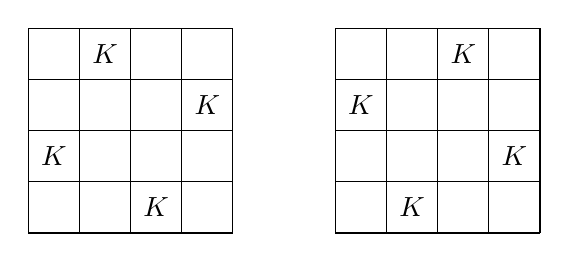
\begin{tikzpicture}[scale=.65]
  \begin{scope}
    \draw (0, 0) grid (4, 4);
    \node at (1.5,3.5) {$K$};
    \node at (3.5,2.5) {$K$};
    \node at (0.5,1.5) {$K$};
    \node at (2.5,0.5) {$K$};

    \draw (6, 0) grid (10, 4);
    \node at (6+2.5,3.5) {$K$};
    \node at (6+0.5,2.5) {$K$};
    \node at (6+3.5,1.5) {$K$};
    \node at (6+1.5,0.5) {$K$};

  \end{scope}
\end{tikzpicture}
\end{center}

The problem can be solved using backtracking
by placing queens to the board row by row.
More precisely, we should place exactly one queen
to each row so that no queen attacks
any of the queens placed before.
A solution is ready when we have placed all
$n$ queens to the board.

For example, when $n=4$, the tree produced by
the backtracking algorithm begins like this:

\begin{center}
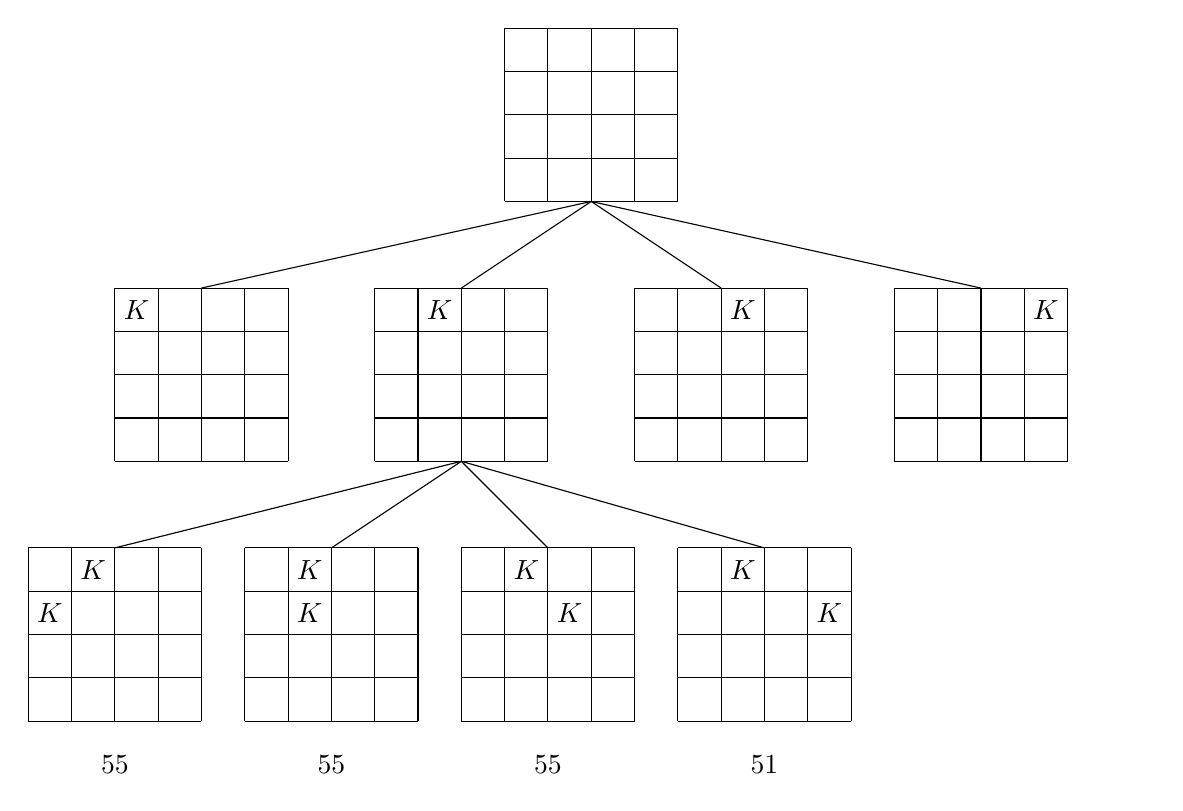
\begin{tikzpicture}[scale=.55]
  \begin{scope}
    \draw (0, 0) grid (4, 4);

    \draw (-9, -6) grid (-5, -2);
    \draw (-3, -6) grid (1, -2);
    \draw (3, -6) grid (7, -2);
    \draw (9, -6) grid (13, -2);

    \node at (-9+0.5,-3+0.5) {$K$};
    \node at (-3+1+0.5,-3+0.5) {$K$};
    \node at (3+2+0.5,-3+0.5) {$K$};
    \node at (9+3+0.5,-3+0.5) {$K$};

    \draw (2,0) -- (-7,-2);
    \draw (2,0) -- (-1,-2);
    \draw (2,0) -- (5,-2);
    \draw (2,0) -- (11,-2);

    \draw (-11, -12) grid (-7, -8);
    \draw (-6, -12) grid (-2, -8);
    \draw (-1, -12) grid (3, -8);
    \draw (4, -12) grid (8, -8);
    \draw[white] (11, -12) grid (15, -8);
    \node at (-11+1+0.5,-9+0.5) {$K$};
    \node at (-6+1+0.5,-9+0.5) {$K$};
    \node at (-1+1+0.5,-9+0.5) {$K$};
    \node at (4+1+0.5,-9+0.5) {$K$};
    \node at (-11+0+0.5,-10+0.5) {$K$};
    \node at (-6+1+0.5,-10+0.5) {$K$};
    \node at (-1+2+0.5,-10+0.5) {$K$};
    \node at (4+3+0.5,-10+0.5) {$K$};

    \draw (-1,-6) -- (-9,-8);
    \draw (-1,-6) -- (-4,-8);
    \draw (-1,-6) -- (1,-8);
    \draw (-1,-6) -- (6,-8);

    \node at (-9,-13) {\ding{55}};
    \node at (-4,-13) {\ding{55}};
    \node at (1,-13) {\ding{55}};
    \node at (6,-13) {\ding{51}};

  \end{scope}
\end{tikzpicture}
\end{center}

At the bottom level, the three first subsolutions
are not valid because the queens attack each other.
However, the fourth subsolution is valid
and it can be extended to a full solution by
placing two more queens to the board.

\begin{samepage}
The following code implements the search:
\begin{lstlisting}
void search(int y) {
    if (y == n) {
        c++;
        return;
    }
    for (int x = 0; x < n; x++) {
        if (r1[x] || r2[x+y] || r3[x-y+n-1]) continue;
        r1[x] = r2[x+y] = r3[x-y+n-1] = 1;
        search(y+1);
        r1[x] = r2[x+y] = r3[x-y+n-1] = 0;
    }
}
\end{lstlisting}
\end{samepage}
The search begins by calling \texttt{search(0)}.
The size of the board is in the variable $n$,
and the code calculates the number of solutions
to the variable $c$.

The code assumes that the rows and columns
of the board are numbered from 0.
The function places a queen to row $y$
when $0 \le y < n$.
Finally, if $y=n$, one solution has been found
and the variable $c$ is increased by one.

The array \texttt{r1} keeps track of the columns
that already contain a queen.
Similarly, the arrays \texttt{r2} and \texttt{r3}
keep track of the diagonals.
It is not allowed to add another queen to a
column or to a diagonal. 
For example, the rows and the diagonals of
the $4 \times 4$ board are numbered as follows:

\begin{center}
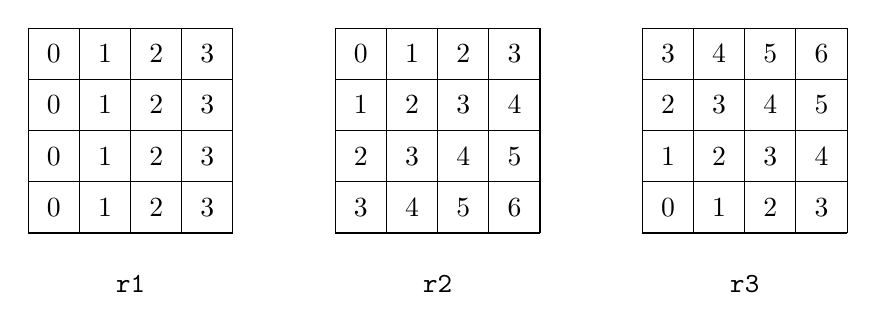
\begin{tikzpicture}[scale=.65]
  \begin{scope}
    \draw (0-6, 0) grid (4-6, 4);
    \node at (-6+0.5,3.5) {$0$};
    \node at (-6+1.5,3.5) {$1$};
    \node at (-6+2.5,3.5) {$2$};
    \node at (-6+3.5,3.5) {$3$};
    \node at (-6+0.5,2.5) {$0$};
    \node at (-6+1.5,2.5) {$1$};
    \node at (-6+2.5,2.5) {$2$};
    \node at (-6+3.5,2.5) {$3$};
    \node at (-6+0.5,1.5) {$0$};
    \node at (-6+1.5,1.5) {$1$};
    \node at (-6+2.5,1.5) {$2$};
    \node at (-6+3.5,1.5) {$3$};
    \node at (-6+0.5,0.5) {$0$};
    \node at (-6+1.5,0.5) {$1$};
    \node at (-6+2.5,0.5) {$2$};
    \node at (-6+3.5,0.5) {$3$};

    \draw (0, 0) grid (4, 4);
    \node at (0.5,3.5) {$0$};
    \node at (1.5,3.5) {$1$};
    \node at (2.5,3.5) {$2$};
    \node at (3.5,3.5) {$3$};
    \node at (0.5,2.5) {$1$};
    \node at (1.5,2.5) {$2$};
    \node at (2.5,2.5) {$3$};
    \node at (3.5,2.5) {$4$};
    \node at (0.5,1.5) {$2$};
    \node at (1.5,1.5) {$3$};
    \node at (2.5,1.5) {$4$};
    \node at (3.5,1.5) {$5$};
    \node at (0.5,0.5) {$3$};
    \node at (1.5,0.5) {$4$};
    \node at (2.5,0.5) {$5$};
    \node at (3.5,0.5) {$6$};

    \draw (6, 0) grid (10, 4);
    \node at (6.5,3.5) {$3$};
    \node at (7.5,3.5) {$4$};
    \node at (8.5,3.5) {$5$};
    \node at (9.5,3.5) {$6$};
    \node at (6.5,2.5) {$2$};
    \node at (7.5,2.5) {$3$};
    \node at (8.5,2.5) {$4$};
    \node at (9.5,2.5) {$5$};
    \node at (6.5,1.5) {$1$};
    \node at (7.5,1.5) {$2$};
    \node at (8.5,1.5) {$3$};
    \node at (9.5,1.5) {$4$};
    \node at (6.5,0.5) {$0$};
    \node at (7.5,0.5) {$1$};
    \node at (8.5,0.5) {$2$};
    \node at (9.5,0.5) {$3$};

    \node at (-4,-1) {\texttt{r1}};
    \node at (2,-1) {\texttt{r2}};
    \node at (8,-1) {\texttt{r3}};

  \end{scope}
\end{tikzpicture}
\end{center}

Using the presented backtracking
algorithm, we can calculate that,
for example, there are 92 ways to place 8
queens to an $8 \times 8$ chessboard.
When $n$ increases, the search quickly becomes slow
because the number of the solutions increases
exponentially.
For example, calculating the ways to
place 16 queens to the $16 \times 16$
chessboard already takes about a minute
(there are 14772512 solutions).

\section{Pruning the search}

A backtracking algorithm can often be optimized
by pruning the search tree.
The idea is to add ''intelligence'' to the algorithm
so that it will notice as soon as possible
if is not possible to extend a subsolution into
a full solution.
This kind of optimization can have a tremendous
effect on the efficiency of the search.

Let us consider a problem where
our task is to calculate the number of paths
in an $n \times n$ grid from the upper-left corner
to the lower-right corner so that each square
will be visited exactly once.
For example, in the $7 \times 7$ grid,
there are 111712 possible paths from the
lower-right corner to the upper-right corner.
One of the paths is as follows:

\begin{center}
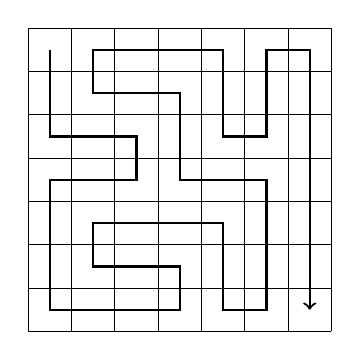
\begin{tikzpicture}[scale=.55]
  \begin{scope}
    \draw (0, 0) grid (7, 7);
    \draw[thick,->] (0.5,6.5) -- (0.5,4.5) -- (2.5,4.5) --
          (2.5,3.5) -- (0.5,3.5) -- (0.5,0.5) --
          (3.5,0.5) -- (3.5,1.5) -- (1.5,1.5) --
          (1.5,2.5) -- (4.5,2.5) -- (4.5,0.5) --
          (5.5,0.5) -- (5.5,3.5) -- (3.5,3.5) --
          (3.5,5.5) -- (1.5,5.5) -- (1.5,6.5) --
          (4.5,6.5) -- (4.5,4.5) -- (5.5,4.5) --
          (5.5,6.5) -- (6.5,6.5) -- (6.5,0.5);
  \end{scope}
\end{tikzpicture}
\end{center}

We will concentrate on the $7 \times 7$ case
because it is computationally suitable difficult.
We begin with a straightforward backtracking algorithm,
and then optimize it step by step using observations
how the search tree can be pruned.
After each optimization, we measure the running time
of the algorithm and the number of recursive calls,
so that we will clearly see the effect of each
optimization on the efficiency of the search.

\subsubsection{Basic algorithm}

The first version of the algorithm doesn't contain
any optimizations. We simply use backtracking to generate
all possible paths from the upper-left corner to
the lower-right corner.

\begin{itemize}
\item
running time: 483 seconds
\item
recursive calls: 76 billions
\end{itemize}

\subsubsection{Optimization 1}

The first step in a solution is either
downward or to the right.
There are always two paths that 
are symmetric
about the diagonal of the grid
after the first step.
For example, the following paths are symmetric:

\begin{center}
\begin{tabular}{ccc}
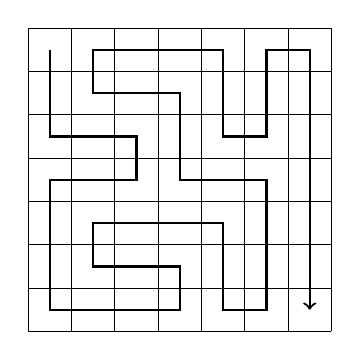
\begin{tikzpicture}[scale=.55]
  \begin{scope}
    \draw (0, 0) grid (7, 7);
    \draw[thick,->] (0.5,6.5) -- (0.5,4.5) -- (2.5,4.5) --
          (2.5,3.5) -- (0.5,3.5) -- (0.5,0.5) --
          (3.5,0.5) -- (3.5,1.5) -- (1.5,1.5) --
          (1.5,2.5) -- (4.5,2.5) -- (4.5,0.5) --
          (5.5,0.5) -- (5.5,3.5) -- (3.5,3.5) --
          (3.5,5.5) -- (1.5,5.5) -- (1.5,6.5) --
          (4.5,6.5) -- (4.5,4.5) -- (5.5,4.5) --
          (5.5,6.5) -- (6.5,6.5) -- (6.5,0.5);
  \end{scope}
\end{tikzpicture}
& \hspace{20px}
& 
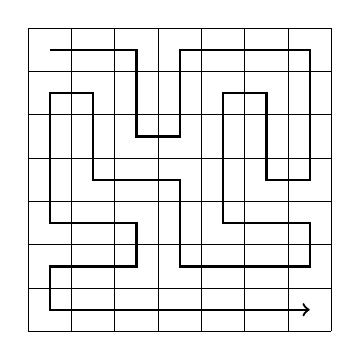
\begin{tikzpicture}[scale=.55]
  \begin{scope}[yscale=1,xscale=-1,rotate=-90]
    \draw (0, 0) grid (7, 7);
    \draw[thick,->] (0.5,6.5) -- (0.5,4.5) -- (2.5,4.5) --
          (2.5,3.5) -- (0.5,3.5) -- (0.5,0.5) --
          (3.5,0.5) -- (3.5,1.5) -- (1.5,1.5) --
          (1.5,2.5) -- (4.5,2.5) -- (4.5,0.5) --
          (5.5,0.5) -- (5.5,3.5) -- (3.5,3.5) --
          (3.5,5.5) -- (1.5,5.5) -- (1.5,6.5) --
          (4.5,6.5) -- (4.5,4.5) -- (5.5,4.5) --
          (5.5,6.5) -- (6.5,6.5) -- (6.5,0.5);
  \end{scope}
\end{tikzpicture}
\end{tabular}
\end{center}

Thus, we can decide that the first step
in the solution is always downward,
and finally multiply the number of the solutions by two.

\begin{itemize}
\item
running time: 244 seconds
\item
recursive calls: 38 billions
\end{itemize}

\subsubsection{Optimization 2}

If the path reaches the lower-right square
before it has visited all other squares of the grid,
it is clear that
it will not be possible to complete the solution.
An example of this is the following case:

\begin{center}
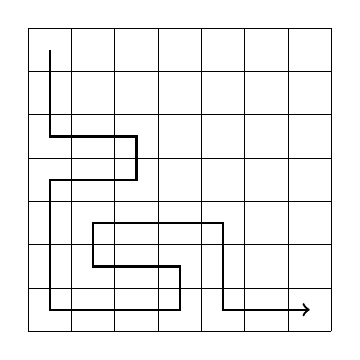
\begin{tikzpicture}[scale=.55]
  \begin{scope}
    \draw (0, 0) grid (7, 7);
    \draw[thick,->] (0.5,6.5) -- (0.5,4.5) -- (2.5,4.5) --
          (2.5,3.5) -- (0.5,3.5) -- (0.5,0.5) --
          (3.5,0.5) -- (3.5,1.5) -- (1.5,1.5) --
          (1.5,2.5) -- (4.5,2.5) -- (4.5,0.5) --
          (6.5,0.5);
  \end{scope}
\end{tikzpicture}
\end{center}
Using this observation, we can terminate the search branch
immediately if we reach the lower-right square too early.
\begin{itemize}
\item
running time: 119 seconds
\item
recursive calls: 20 billions
\end{itemize}

\subsubsection{Optimization 3}

If the path touches the wall so that there is
an unvisited square at both sides,
the grid splits into two parts.
For example, in the following case
both the left and the right squares
are unvisited:

\begin{center}
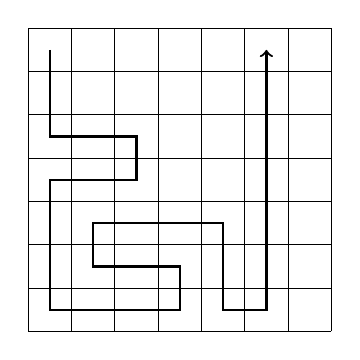
\begin{tikzpicture}[scale=.55]
  \begin{scope}
    \draw (0, 0) grid (7, 7);
    \draw[thick,->] (0.5,6.5) -- (0.5,4.5) -- (2.5,4.5) --
          (2.5,3.5) -- (0.5,3.5) -- (0.5,0.5) --
          (3.5,0.5) -- (3.5,1.5) -- (1.5,1.5) --
          (1.5,2.5) -- (4.5,2.5) -- (4.5,0.5) --
          (5.5,0.5) -- (5.5,6.5);
  \end{scope}
\end{tikzpicture}
\end{center}
Now it will not be possible to visit every square,
so we can terminate the search branch.
This optimization is very useful:

\begin{itemize}
\item
running time: 1.8 seconds
\item
recursive calls: 221 millions
\end{itemize}

\subsubsection{Optimization 4}

The idea of the previous optimization
can be generalized:
the grid splits into two parts
if the top and bottom neighbors
of the current square are unvisited and
the left and right neighbors are
wall or visited (or vice versa).

For example, in the following case
the top and bottom neighbors are unvisited,
so the path cannot visit all squares
in the grid anymore:
\begin{center}
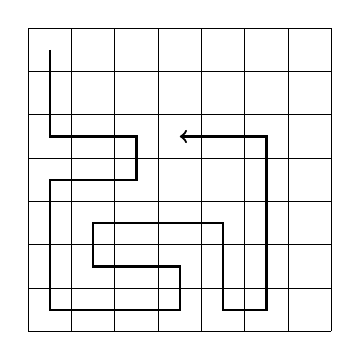
\begin{tikzpicture}[scale=.55]
  \begin{scope}
    \draw (0, 0) grid (7, 7);
    \draw[thick,->] (0.5,6.5) -- (0.5,4.5) -- (2.5,4.5) --
          (2.5,3.5) -- (0.5,3.5) -- (0.5,0.5) --
          (3.5,0.5) -- (3.5,1.5) -- (1.5,1.5) --
          (1.5,2.5) -- (4.5,2.5) -- (4.5,0.5) --
          (5.5,0.5) -- (5.5,4.5) -- (3.5,4.5);
  \end{scope}
\end{tikzpicture}
\end{center}
The search becomes even faster when we terminate
the search branch in all such cases:

\begin{itemize}
\item
running time: 0.6 seconds
\item
recursive calls: 69 millions
\end{itemize}

~\\
Now it's a good moment to stop optimization
and remember our starting point.
The running time of the original algorithm
was 483 seconds,
and now after the optimizations,
the running time is only 0.6 seconds.
Thus, the algorithm became nearly 1000 times
faster after the optimizations.

This is a usual phenomenon in backtracking
because the search tree is usually large
and even simple optimizations can prune
a lot of branches in the tree.
Especially useful are optimizations that
occur at the top of the search tree because
they can prune the search very efficiently.

\section{Meet in the middle}

\index{meet in the middle}

\key{Meet in the middle} is a technique
where the search space is divided into
two equally large parts.
A separate search is performed
for each of the parts,
and finally the results of the searches are combined.

The meet in the middle technique can be used
if there is an efficient way to combine the
results of the searches.
In this case, the two searches may require less
time than one large search.
Typically, we can turn a factor of $2^n$
into a factor of $2^{n/2}$ using the meet in the
middle technique.

As an example, consider a problem where
we are given a list of $n$ numbers and
an integer $x$.
Our task is to find out if it is possible
to choose some numbers from the list so that
the sum of the numbers is $x$.
For example, given the list $[2,4,5,9]$ and $x=15$,
we can choose the numbers $[2,4,9]$ to get $2+4+9=15$.
However, if the list remains the same but $x=10$,
it is not possible to form the sum.

A standard solution for the problem is to
go through all subsets of the elements and
check if the sum of any of the subsets is $x$.
The time complexity of this solution is $O(2^n)$
because there are $2^n$ possible subsets.
However, using the meet in the middle technique,
we can create a more efficient $O(2^{n/2})$ time solution.
Note that $O(2^n)$ and $O(2^{n/2})$ are different
complexities because $2^{n/2}$ equals $\sqrt{2^n}$.

The idea is to divide the list given as input
to two lists $A$ and $B$ that each contain
about half of the numbers.
The first search generates all subsets
of the numbers in the list $A$ and stores their sums
to list $S_A$.
Correspondingly, the second search creates
the list $S_B$ from the list $B$.
After this, it suffices to check if it is possible
to choose one number from $S_A$ and another
number from $S_B$ so that their sum is $x$.
This is possible exactly when there is a way to
form the sum $x$ using the numbers in the original list.

For example, assume that the list is $[2,4,5,9]$ and $x=15$.
First, we divide the list into $A=[2,4]$ and $B=[5,9]$.
After this, we create the lists
$S_A=[0,2,4,6]$ and $S_B=[0,5,9,14]$.
The sum $x=15$ is possible to form
because we can choose the number $6$ from $S_A$
and the number $9$ from $S_B$.
This choice corresponds to the solution $[2,4,9]$.

The time complexity of the algorithm is $O(2^{n/2})$
because both lists $A$ and $B$ contain $n/2$ numbers
and it takes $O(2^{n/2})$ time to calculate the sums of
their subsets to lists $S_A$ and $S_B$.
After this, it is possible to check in 
$O(2^{n/2})$ time if the sum $x$ can be created
using the numbers in $S_A$ and $S_B$.